\documentclass[captions=tableheading]{scrartcl}
\usepackage[aux]{rerunfilecheck}

\usepackage{fontspec}
\usepackage[main=ngerman]{babel}
\usepackage[unicode]{hyperref}
\usepackage{bookmark}
\usepackage{booktabs}
\usepackage{amsmath}
\usepackage{amssymb}
\usepackage{mathtools}
\usepackage{graphicx}
\usepackage{grffile}
\usepackage{scrhack}
\usepackage{float}
\usepackage{pdfpages}
\floatplacement{figure}{htbp}
\setmainfont{Libertinus Serif}
\subject{Versuchsnummer: 303}
\title{Der Lock-In-Verstärker}
\author{Richard Leven \\ \href{mailto:richard.leven@tu-dortmund.de}{richard.leven@tu-dortmund.de}
 \and Joell - D. Jones \\ \href{mailto:joell-david.jones@tu-dortmund.de}{joell-david.jones@tu-dortmund.de}} 
\date{
    Durchführung: 19.11.2019\\
    Abgabe: 26.11.2019
}
\publishers{TU Dortmund - Fachschaft Physik}
\begin{document}
\maketitle
\newpage
\section{Ziel}
Kennenlernen des Lock-In-Verstärkers
\section{Theorie}
Ein Lock-In-Verstärker liefert eine klare Gleichspannung bei einem Input von einem Signal mit Rauschen und einem Referenzsignal.
Zuerst werden die zu hohen und zu niedrigen Frequenzen des rauschenden Nutzsignals mit einem Bandpassfilter eliminiert.
Ein Referenzsignal mit gleicher Phase und Frequenz wird nun mit dem Nutzsignal vermischt.
Das resultierende Signal wird mit einem Tiefpassfilter integriert, sodass eine Gleichspannung erzeugt wird, die rauschfrei ist.
\section{Aufgaben}
    \begin{itemize}
        \item{Aufgabe 1 \\}
        Kennenlernen des Schaltkreises des Lock-In-Verstärkers und Ermittlung des konstanten Spannungs-Outputs und variablen Spannungs-Outputs.
        \item{Aufgabe 2 \\}
        Ausgangssignal für 5 verschiedene Phasen messen, mit ausgeschaltetem Noise-Generator.
        \item{Aufgabe 3 \\}
        Wie Aufgabe 2, nur mit Noise-Generator.
        \item{Aufgabe 4 \\}
        Nachweisen eines maximalen Abstandes \(r_{max}\) , in der die Photodiode das Licht einer LED noch messen kann.
        Aufstellen einer Funktion, die die Intensität in Abhängigkeit von \(r\) zeigt.
    \end{itemize}
\section{Versuchsaufbau}

\begin{figure}
\centering
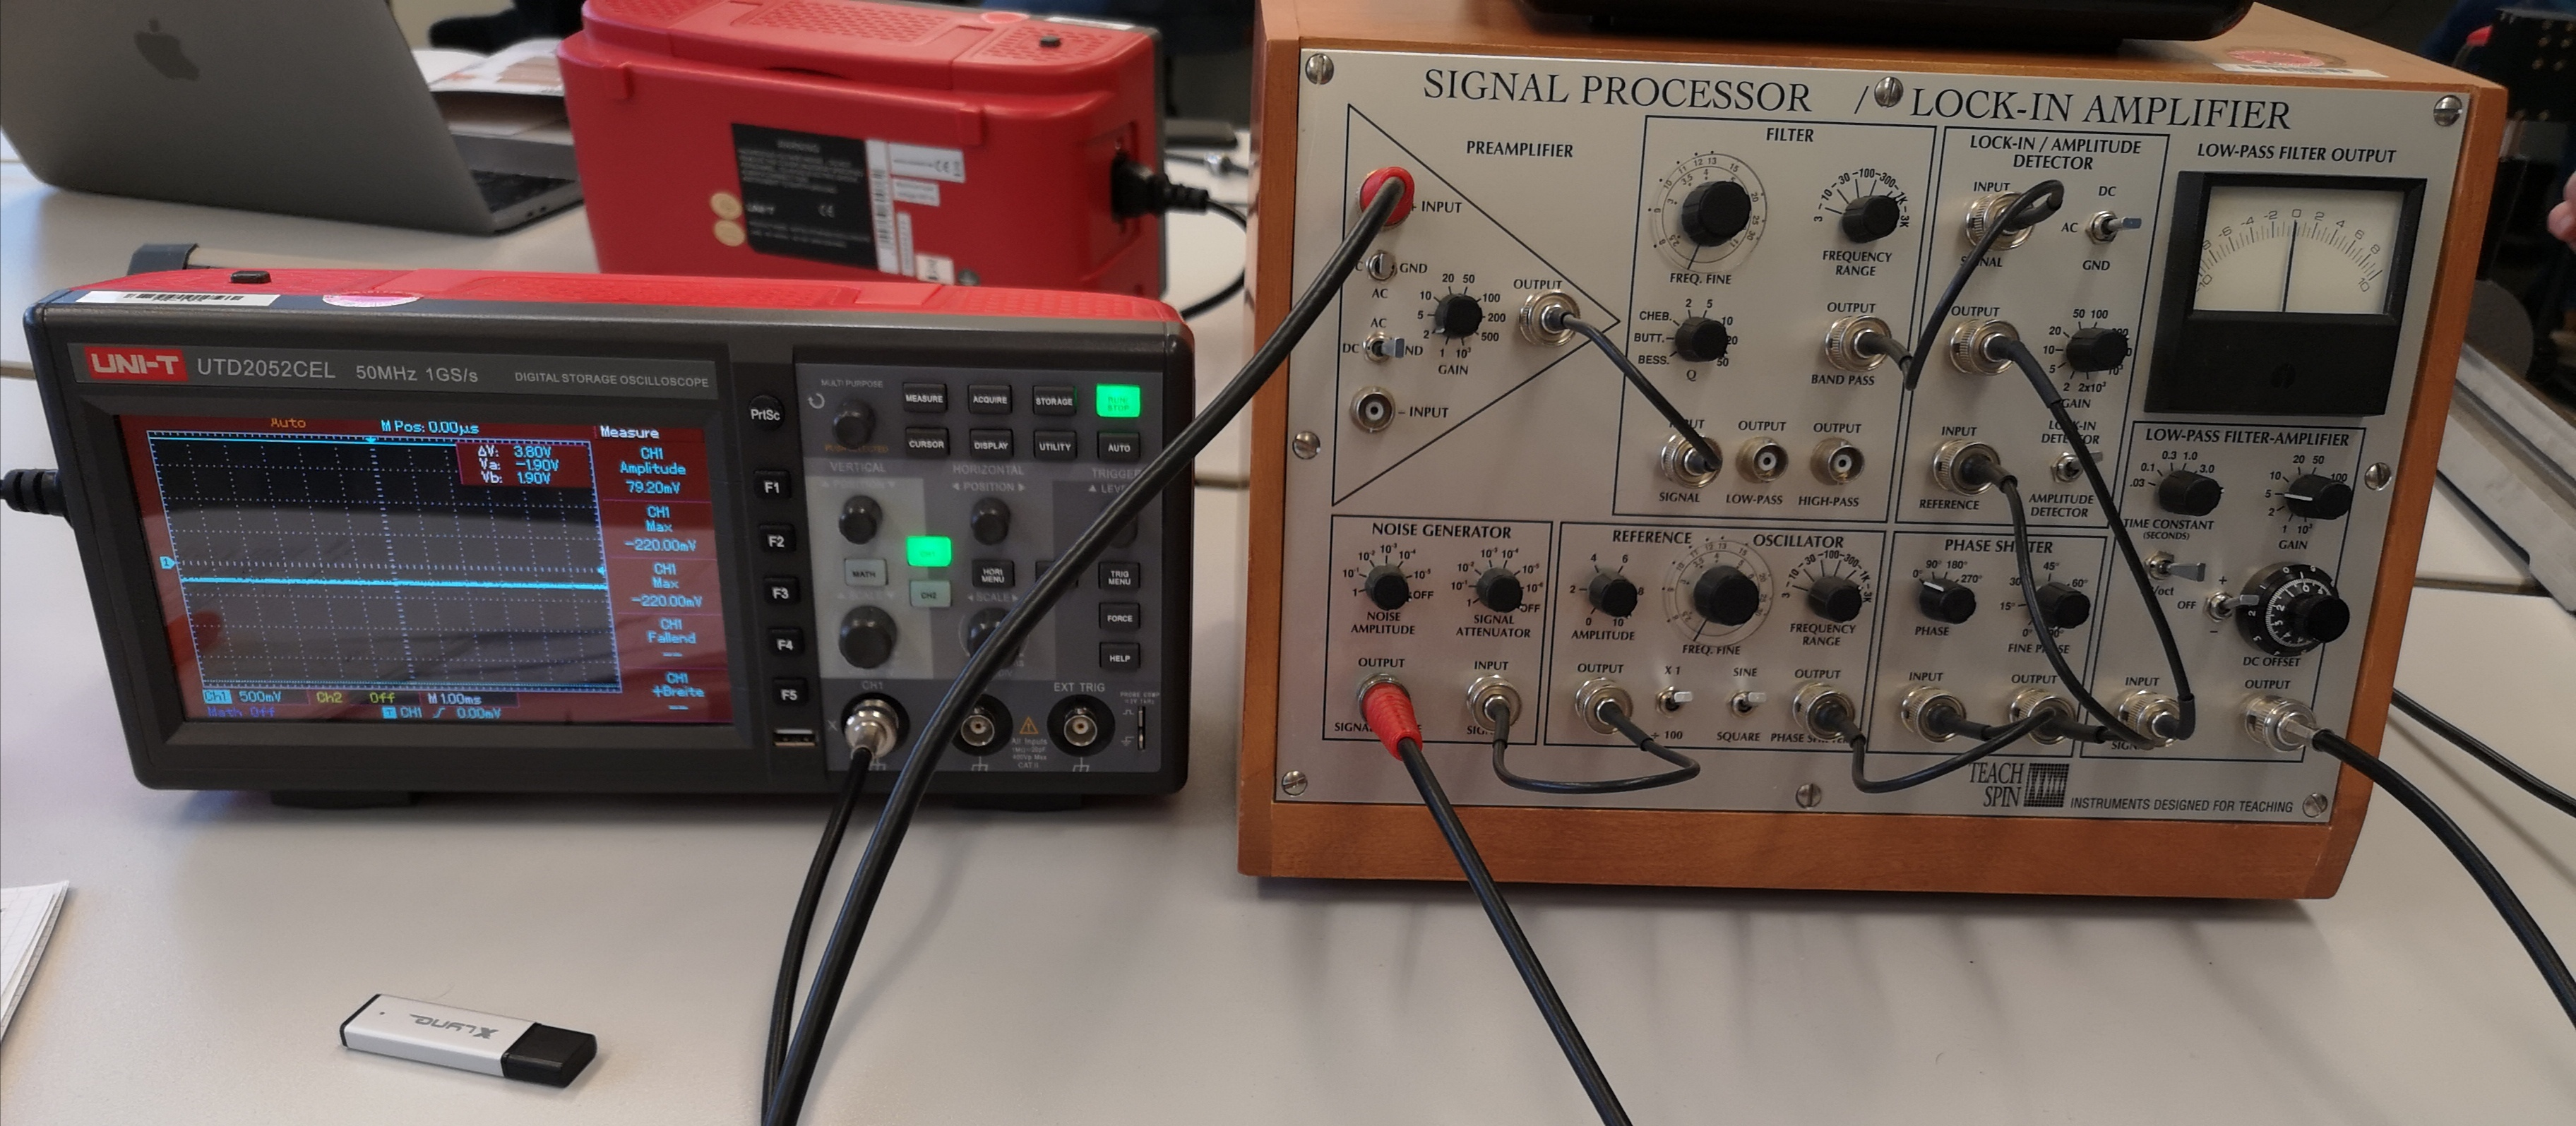
\includegraphics[scale=0.07]{Lock_In Bilder/Versauf.jpg}
\caption{Der Versuchsaufbau}
\label{fig:versau}
\end{figure}
\newpage
\section{Versuchsdurchführung}
In Aufgabe 1 wurden die Outputs am Lock-In-Verstärker variiert, sodass einmal der Tiefpass überbrückt wurde und einmal nicht.
Die Outputs wurden an das Oszilloskop angeschlossen und an den Bildschirm angepasst, um ein klares Bild zu bekommen.
\\ \\
In Aufgabe 2 wurde der Tiefpass erneut überbrückt und fünf verschiedene Phaseneinstellungen eingestellt: \(0°, 45°, 90°, 135°, 180°\) \\
Die resultierenden Signale sind in der Auswertung zu sehen.
\\ \\
In Aufgabe 3 wurde das Rauschen auf $10^{-3}$ eingestellt, was der Größenordnung der Spannung des Signals entsprach.
Es wurden danach die gleichen Phasen, wie bei Aufgabe 2 eingestellt.
Die resultierenden Signale sind in der Auswertung zu sehen.
\\ \\
In Aufgabe 4 wurde der Schaltkreis leicht modifiziert, sodass nun der Output vom Lock-In-Verstärker nicht mehr nach dem Tiefpass erfolgte, 
sondern bereits nach dem Lock-In. 
Gleichzeitig wurde auch ein Signal zum Tiefpass-Input gelegt, sodass der Versuchsaufbau nun wie die Schaltkreis-Skizze der Aufgabe 4 geschaltet war.
Die LED wurde mit einer Frequenz von 300Hz betrieben. 
Für eine genauere Messung wurde der Raum verdunkelt und teilweise wurde das Experiment mit Objekten zugedeckt.
\newpage
\section{Auswertung}
    \begin{itemize}
        \item{Aufgabe 1 \\}
            \begin{figure}
                \centering
                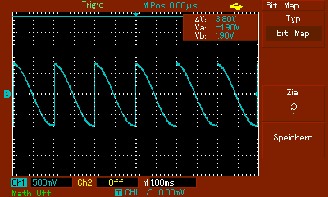
\includegraphics{Lock_In Bilder/Aufgabe 1/MAP001.pdf}
                \caption{Die Sägezahnschwingung}
                \label{fig:sawsig}
            \end{figure}
            \\
            In Abbildung \ref{fig:sawsig} wurde der Output nach dem Lock-In abgegriffen und nicht nach dem Tiefpass.
            Eine Sägezahnschwingung ist das Resultat. 
            \\
            \begin{figure}
                \centering
                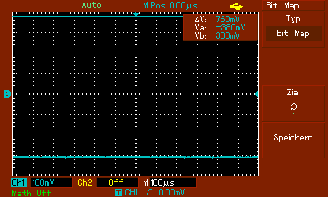
\includegraphics{Lock_In Bilder/Aufgabe 1/MAP002.pdf}
                \caption{Die Gleichspannung}
                \label{fig:flatsig}
            \end{figure}
            \\
            In Abbildung \ref{fig:flatsig} wurde der Output nach dem Tiefpass abgegriffen.
            Eine Gleichspannung im negativen Bereich ist das Resultat.
            Sie entsteht, wenn die Sägezahnschwingung aus Abbildung \ref{fig:sawsig} durch den Tiefpass verändert wird.
        \newpage
        \item{Aufgabe 2 \\}
            \begin{itemize}
            \item{0° Phase}
            \begin{figure}
                \centering
                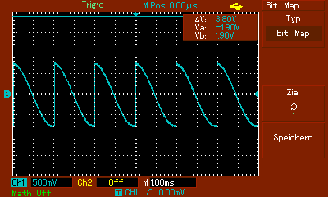
\includegraphics{Lock_In Bilder/Aufgabe 2/MAP001.pdf}
                \caption{AC-Signal bei 0° Phase}
                \label{fig:0sig}
            \end{figure}
            \\
            \item{45° Phase}
            \begin{figure}
                \centering
                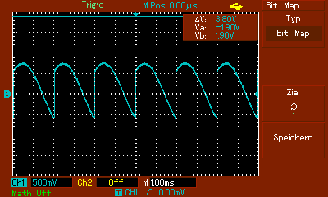
\includegraphics{Lock_In Bilder/Aufgabe 2/MAP002.pdf}
                \caption{AC-Signal bei 45° Phase}
                \label{fig:45sig}
            \end{figure}
            \\
            \item{90° Phase}
            \begin{figure}
                \centering
                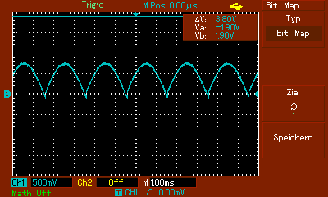
\includegraphics{Lock_In Bilder/Aufgabe 2/MAP003.pdf}
                \caption{AC-Signal bei 90° Phase}
                \label{fig:90sig}
            \end{figure}
            \\
            \newpage
            \item{135° Phase}
            \begin{figure}
                \centering
                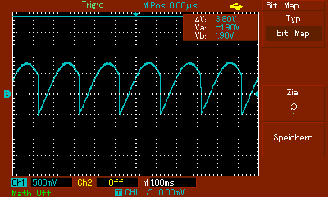
\includegraphics{Lock_In Bilder/Aufgabe 2/MAP004.pdf}
                \caption{AC-Signal bei 135° Phase}
                \label{fig:135sig}
            \end{figure}
            \\
            \item{180° Phase}
            \begin{figure}
                \centering
                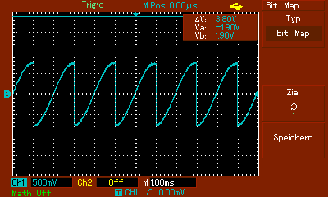
\includegraphics{Lock_In Bilder/Aufgabe 2/MAP005.pdf}
                \caption{AC-Signal bei 180° Phase}
                \label{fig:180sig}
            \end{figure}
            \\
            Die Signale entsprechen der theoretischen Vorstellung, wenn \(U_{ref}\) um die jeweiligen Grade verschoben wird.
            \end{itemize}
        \newpage
        \item{Aufgabe 3 \\}
            \begin{itemize}
            \item{0° Phase}
            \begin{figure}
                \centering
                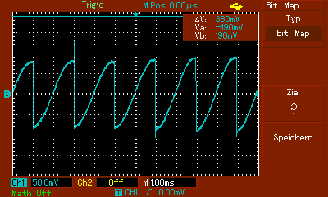
\includegraphics{Lock_In Bilder/Aufgabe 3/MAP001.pdf}
                \caption{AC-Signal bei 0° Phase}
                \label{fig:0sig2}
            \end{figure}
            \\
            \item{45° Phase}
            \begin{figure}
                \centering
                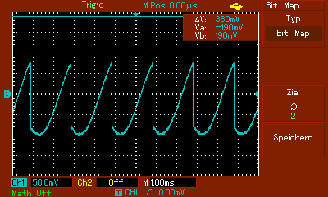
\includegraphics{Lock_In Bilder/Aufgabe 3/MAP002.pdf}
                \caption{AC-Signal bei 45° Phase}
                \label{fig:45sig2}
            \end{figure}
            \\
            \item{90° Phase}
            \begin{figure}
                \centering
                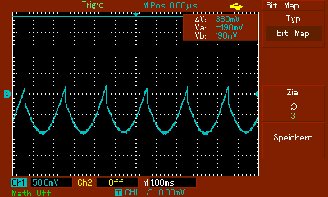
\includegraphics{Lock_In Bilder/Aufgabe 3/MAP003.pdf}
                \caption{AC-Signal bei 90° Phase}
                \label{fig:90sig2}
            \end{figure}
            \\
            \newpage
            \item{135° Phase}
            \begin{figure}
                \centering
                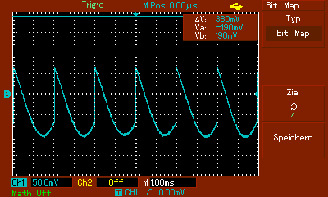
\includegraphics{Lock_In Bilder/Aufgabe 3/MAP004.pdf}
                \caption{AC-Signal bei 135° Phase}
                \label{fig:135sig2}
            \end{figure}
            \\
            \item{180° Phase}
            \begin{figure}
                \centering
                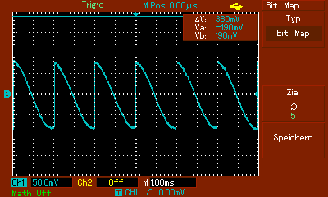
\includegraphics{Lock_In Bilder/Aufgabe 3/MAP005.pdf}
                \caption{AC-Signal bei 180° Phase}
                \label{fig:180sig2}
            \end{figure}
            \\
            \end{itemize}
        \item{Aufgabe 4 \\}
        \\
            \begin{figure}
                \centering
                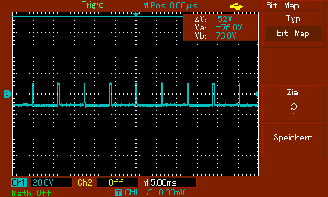
\includegraphics{Lock_In Bilder/Aufgabe 4/MAP001.pdf}
                \caption{Signal bei 5cm}
                \label{fig:5cmled}
            \end{figure}  
            \\
            \begin{figure}   
                \centering 
                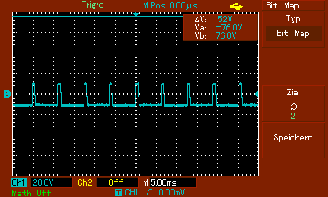
\includegraphics{Lock_In Bilder/Aufgabe 4/MAP002.pdf}
                \caption{Signal bei 10cm}
                \label{fig:10cmled}
            \end{figure}   
            \\
            \begin{figure}    
                \centering
                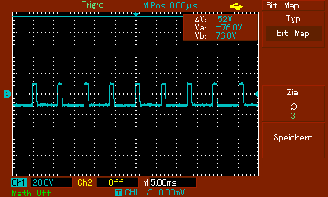
\includegraphics{Lock_In Bilder/Aufgabe 4/MAP003.pdf}
                \caption{Signal bei 15cm}
                \label{fig:15cmled}
            \end{figure}   
            \\
            \begin{figure} 
                \centering  
                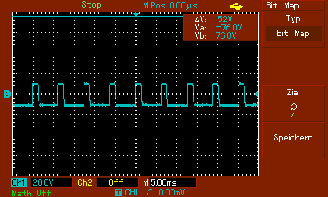
\includegraphics{Lock_In Bilder/Aufgabe 4/MAP004.pdf}
                \caption{Signal bei 20cm}
                \label{fig:20cmled}    
            \end{figure}
            \\
        Die sich vergrößernden Abstände in den Signalen in Mikrosekunden zeigen die Abschwächung des Lichtsignals. (Siehe Diskussion)
            \begin{figure}
                \centering
                \includegraphics[scale=0.75]{build/graph.pdf}
                \caption{Messwerte des LED-Abstands}
                \label{fig:graph}
            \end{figure}
        \\
        Hier ist eine Veranschaulichung der Messwerte und ihrer Korrelation zu einem \(1/r²\) Abstand.
    \end{itemize}
\section{Diskussion}
Der Unterschied zwischen den Messungen in Aufgabe 1 resultiert aus der Tatsache, dass der Tiefpass den Strom hier, in diesem Fall, mit nur einem bestimmten Frequenzbereich durchlässt. Von daher entsteht ein Gleichstrom.
Die durch den Bandpass erzwungene Sägezahnkurve entsteht aus der Überlagerung von \(U_{ref}\) und \(U_{sig}\).
In den Bildern der 2. und 3. Aufgabe scheint die Kurve sich zu spiegeln. Dies entspricht den Erwartungen, da der Phasenunterschied zwischen \(U_{ref}\) und \(U_{sig}\) sich um genau 180 Grad verschiebt und nach Gleichung (5) ändert sich auch das Vorzeichen von der Gesamtspannung.
In der 4. Aufgabe wurden vier richtige und drei falsch gemessene Messungen aufgenommen, welche sich im Anhang befinden.
Die Kurve weist eine \(r²\)-Abhängigkeit auf, weil der durch den Lock-In Verstärker hervorgerufenen Gap in Mikrosekunden als X-Achse gewählt wurde. Diese Gaps werden länger je größer die Distanz zwischen Sender und Empfänger ist. Die Intensität des Lichts weist eine \(1/r²\)-Abhängigkeit auf, wobei sie eben eine Antiproportionalität zu dem, also eine \(r²\)-Abhängigkeit aufweisen.
\newpage
\section{Anhang}
    \begin{figure}
        \centering
        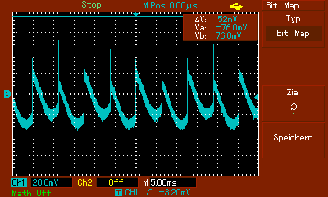
\includegraphics{Lock_In Bilder/Aufgabe 4/Komische Bilder/MAP001.pdf}
        \caption{Falsche Messung Nr.1}
        \label{fig:mismess1}
    \end{figure}
    
    \begin{figure}
        \centering
        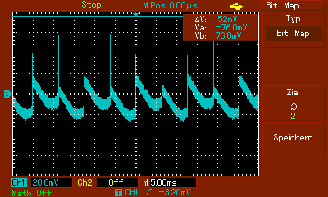
\includegraphics{Lock_In Bilder/Aufgabe 4/Komische Bilder/MAP002.pdf}
        \caption{Falsche Messung Nr.2}
        \label{fig:mismess2}
    \end{figure}
    
    \begin{figure}
        \centering
        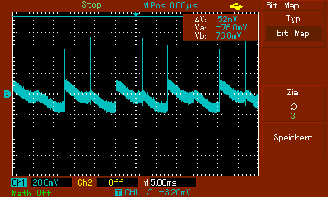
\includegraphics{Lock_In Bilder/Aufgabe 4/Komische Bilder/MAP003.pdf}
        \caption{Falsche Messung Nr.3}
        \label{fig:mismess3}
    \end{figure}

        % Hi Joell! Bitte implementiere hier Aufgabe 3 [Freitag]! Deine Parts sind dann nur noch die Diskussion[Samstag], die Literatur(welche wir nicht haben) [Sonntag] und der Anhang mit den Originaldaten!
        % Ich implementiere Aufgabe 4. Falls dir Verbesserungen einfallen, bitte füge sie ein und sag mir Bescheid :)
        %In die Diskussion muss auf jeden Fall die Begründung rein, warum in graph.pdf eine Korrelation zwischen messwerten und r² ist und nicht 1/r²!!! Das ist weil wir einen Unterschied im signal haben, der in mikrosekunden angezeigt wird und nicht in cm!

        %Richipupsi stinkt!!
\end{document}